\documentclass[11pt,a4paper,notitlepage,onecolumn]{article}
\usepackage[german]{babel}
\usepackage[utf8]{inputenc}
\usepackage{graphicx}
\title{Aufgabe2\_3}
\author{Robin Nehls, Yves Müller\\
  Freie Universit\"at Berlin\\
  nehls@spline.de uves@spline.de }
\date{}
\begin{document}

\maketitle

\paragraph{}
The first plot is done by using only 5 interpolation values, which seems 
to be too few values to get an good result. Also with that few values, the
linear distribution gives better results, because there is no extrem 
behaviour on the far sites of the range. 

\begin{figure}
\centering
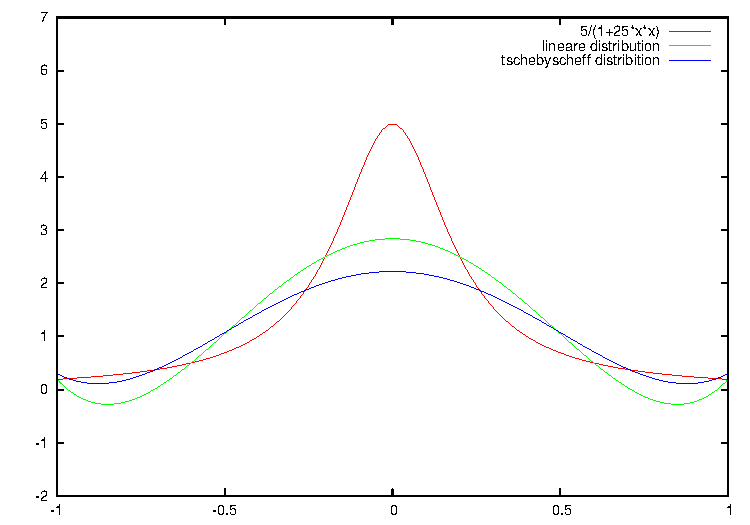
\includegraphics[width=\textwidth]{aufgabe3-2based5.pdf}
\caption{\em \small Results using 5 interpolation values}
\end{figure}


\paragraph{}
With 12 values the function can be better interpolated.

\begin{figure}
\centering
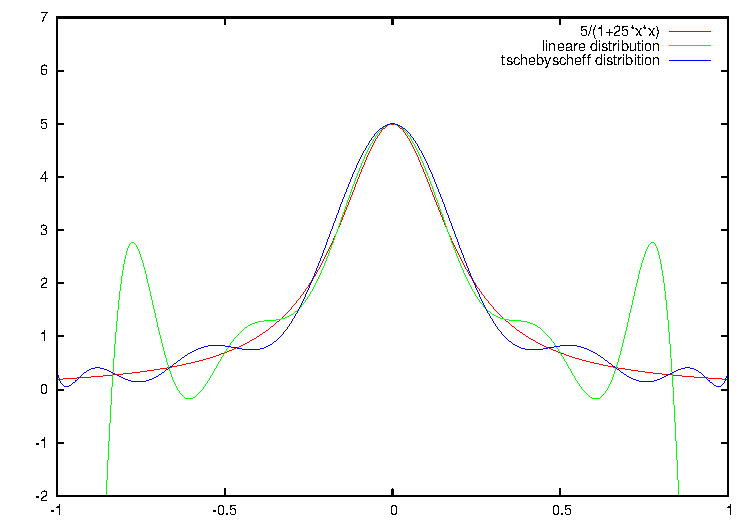
\includegraphics[width=\textwidth]{aufgabe3-2based12.pdf}
\caption{\em \small Results using 12 interpolation values}
\end{figure}


\paragraph{}
With 22 interpoltaion values the tschebyscheff distribution is supperior 
to the lineare distribution. To the range borders, there are more 
interpolation values than in the center, so the extrem behaviour of an
polynomial with degree 20 can be handeled.


\begin{figure}
\centering
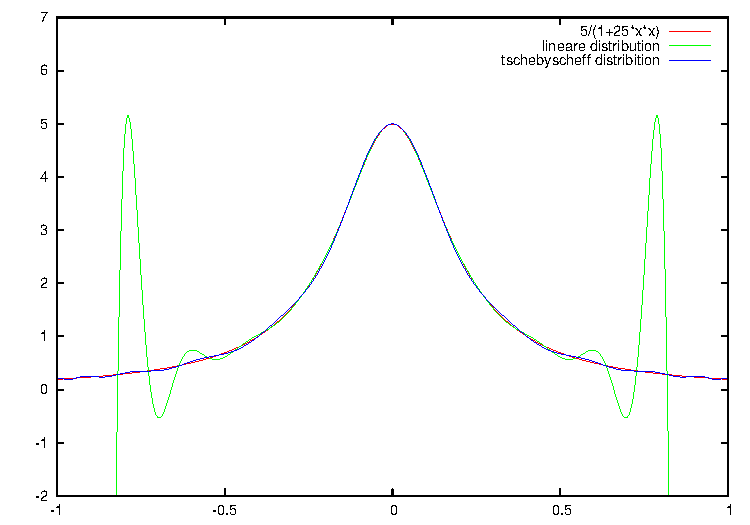
\includegraphics[width=\textwidth]{aufgabe3-2based22.pdf}
\caption{\em \small Results using 22 interpolation values}
\end{figure}
\end{document}
